\chapter{Combined $\htt$ Results}
\label{sec:cmb_results}

The previous two Chapters, ~\ref{sec:htt_analysis} and ~\ref{sec:vh_analysis}, discussed
analyses targeted at specific Higgs boson production mechanisms. In this chapter
I present results from combining the previously mentioned 
$ggH$ and VBF targeted analysis~\cite{cms_13TeV_htt_jhep_2017}
with the $\PW\PH$ and $\PZ\PH$ associated production targeted analysis~\cite{HIG-18-007}.
By combining these two $\htt$ analyses we have signal regions targeting the four leading Higgs 
boson production processes: $ggH$, VBF, and $\PW\PH$ and $\PZ\PH$ associated production. 
By combining the results, signal strengths, significance and, Higgs
boson couplings can be probed with greater precision than either analysis alone.

\section{Signal Strength and Significance}
The best fit signal strength ($\mu$) and significance can be computed for the combination and
result in a decrease in the relative uncertainty on $\mu$ and an increase
in significance. The $\mu$ and significance
for each analysis and the combined values are presented in Table~\ref{tab:cmb_mu_and_sig}.
The slight excess in signal strength for the associated production analysis is tempered
when combined with the $ggH$ and VBF analysis, resulting in a $\mu$ fully consistent 
with the SM. The combination leads to an 
observed significance of 5.5 standard deviations, surpassing the threshold for a
purely 13\TeV based CMS observation of the $\htt$ process.

\begin{table*}[htbp]
\renewcommand{\arraystretch}{1.3}
\centering
\begin{tabular}{lcc}
Analysis         &   Best Fit Signal Strength    &   Observed Significance    \\
\hline
$ggH$ and VBF             &   $\mu = 1.09 ^{+0.27} _{-0.26}$   &  4.9 $\sigma$     \\
Associated production     &   $\mu = 2.5  ^{+1.4}  _{-1.3}$    &  2.3 $\sigma$     \\
$\htt$ combination        &   $\mu = 1.24 ^{+0.29} _{-0.27}$   &  5.5 $\sigma$     \\
\hline
\end{tabular}
\caption{
Best fit signal strength and significance for three fit scenarios: $ggH$ and VBF,
associated production, and the combination.
}
\label{tab:cmb_mu_and_sig}
\end{table*}


The signal strength can be decomposed by the four leading Higgs boson production 
mechanisms. Figure~\ref{fig:cmb_mu_higgs_processes} shows this decomposition for
the combined results. 

\begin{figure}[!ht]
 \begin{center}
  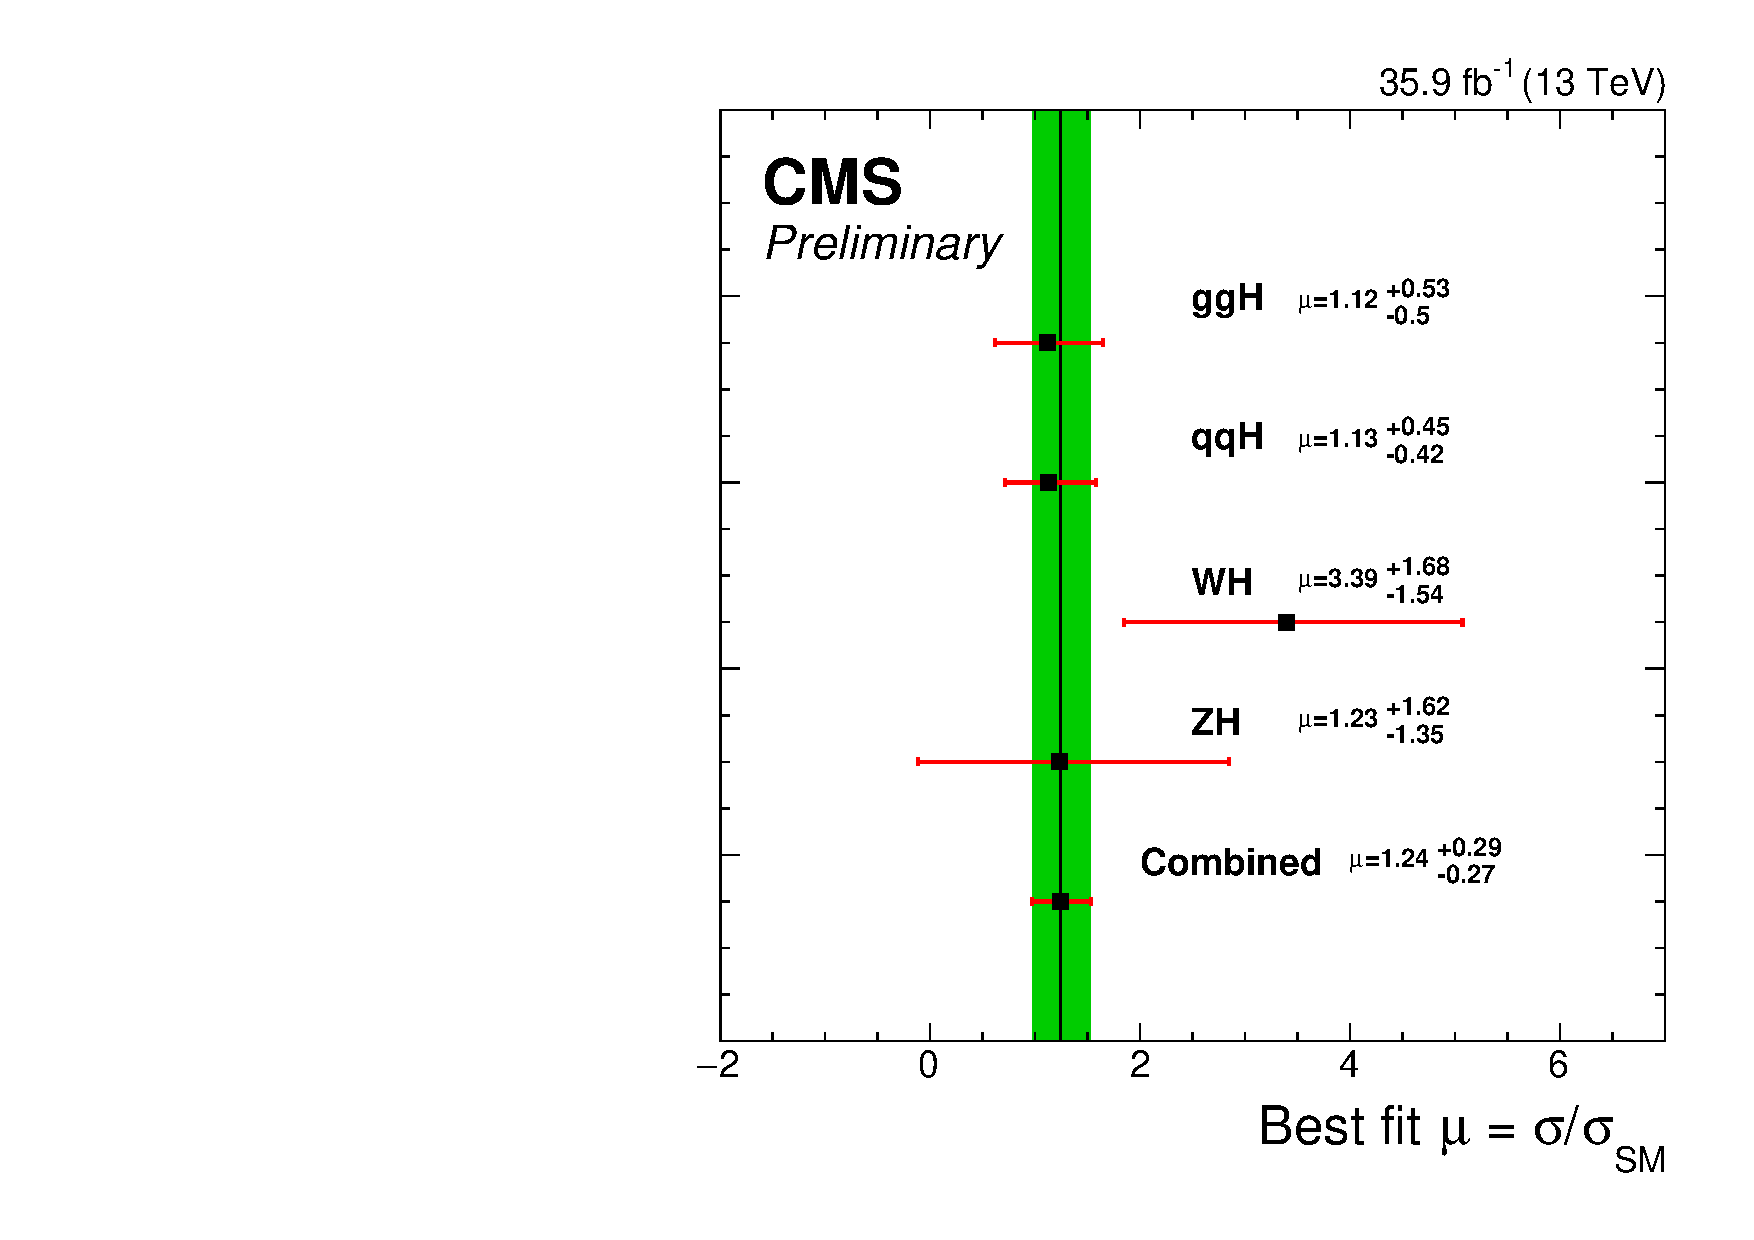
\includegraphics[width=0.65\textwidth]{higgs_to_taus_vh/plots/combined/mu_higgs_procs.pdf}
 \end{center}
 \caption{
 Best fit signal strength per Higgs boson production process, for $\mH = 125.09\GeV$.
 The constraints from the combined global fit are used to extract each of the 
 individual best fit signal strengths. The combined best fit signal strength 
 is $\mu = 1.24 ^{+0.29} _{-0.27}$.
 }
 \label{fig:cmb_mu_higgs_processes}
\end{figure}



\section{Higgs Couplings}
This same combination of the dedicated $ggH$ and VBF analysis with 
the dedicated $\PW\PH$ and $\PZ\PH$ analysis can place the tightest
$\htt$ analysis limits in the $(\kappa_\text{V}$,$\kappa_\text{f})$ parameter space.
$\kappa_\text{V}$ and $\kappa_\text{f}$ quantify, respectively, 
the ratio between the measured and the SM value for the couplings of the Higgs boson to 
vector bosons and fermions using the methods described in Reference~\cite{Khachatryan:2016vau}.
To measure the couplings, a likelihood scan is performed for $\mH=125.09\GeV$ in 
the ($\kappa_\text{V}$,$\kappa_\text{f}$) parameter space.
For this scan only, Higgs boson decays to pairs of $\PW$ or $\PZ$ bosons, $\hww$ or $\hzz$,
are considered as part of the signal. 
%The $\ttbar\PH$ production process is still treated as background because
%the MC sample we use is not split by Higgs boson decay mode. 
All nuisance 
parameters are profiled for each point of the scan. As shown in 
Figure~\ref{fig:cmb_kFkV}, the observed likelihood contour is consistent with the SM expectation 
of $\kappa_\text{V}$ and $\kappa_\text{f}$ both equal to unity.

\begin{figure}[!ht]
 \begin{center}
  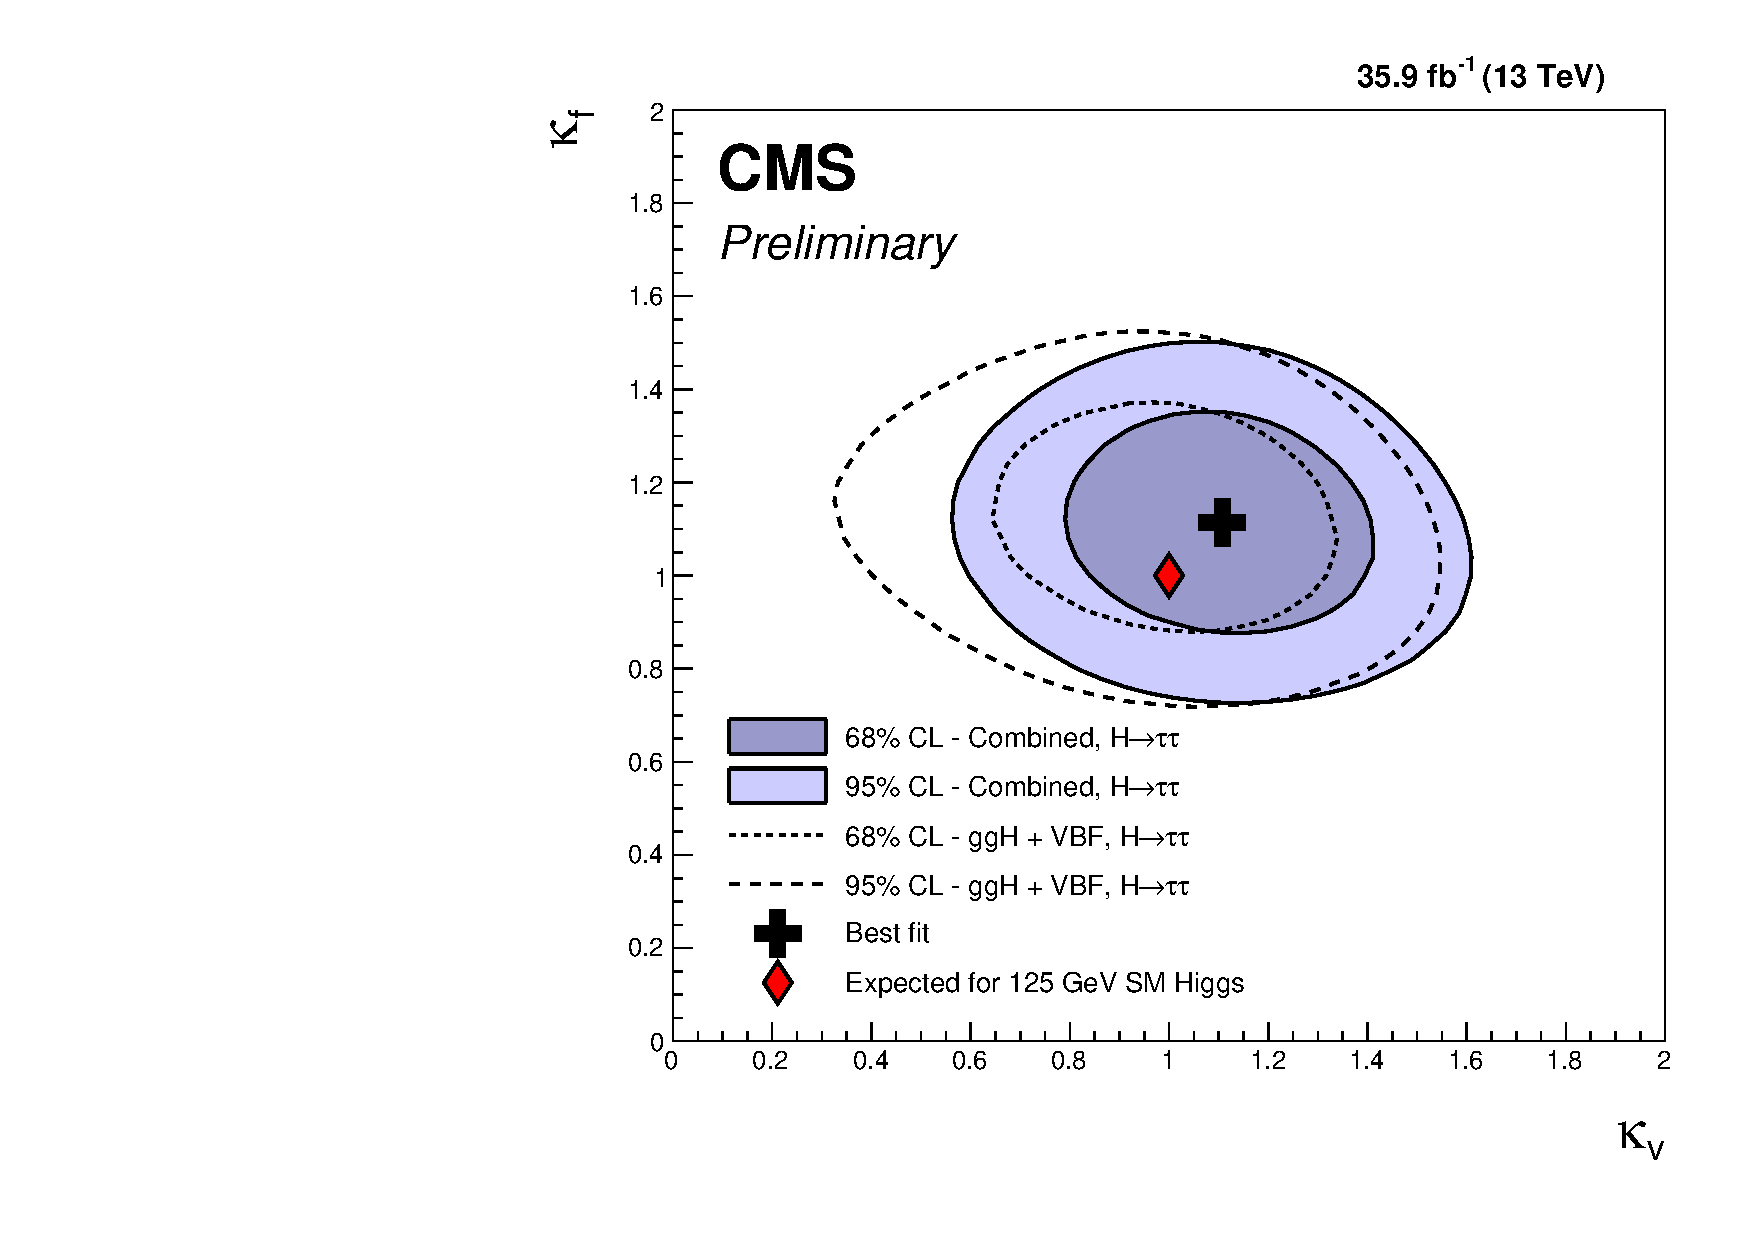
\includegraphics[width=0.60\textwidth]{higgs_to_taus_vh/plots/combined/kFkV_HIG-18-007_plus_HIG-16-043_comp_up.pdf}
 \end{center}
 \caption{Scan of the negative 
 log-likelihood difference as a function of $\kappa_V$ and $\kappa_f$, for 
 $\mH = 125.09$\GeV.  All nuisance parameters are profiled for each point. 
 This scan is a combination of the $ggH$ and VBF targeted analysis with the 
 $\PW\PH$ and $\PZ\PH$ targeted analysis. For reference the results for just
 the $ggH$ and VBF targeted analysis are presented as ``HIG-16-043''.
 For this scan, the $\hww$ and $\hzz$ processes 
 are treated as signal.
 }
 \label{fig:cmb_kFkV}
\end{figure}



\clearpage
